\subsection{UC2 - Errore interpretazione richiesta}
\begin{itemize}
    \item \textbf{Identificativo}: UC2
    \item \textbf{Nome}: Errore interpretazione richiesta
    \item \textbf{Descrione grafica}:
\end{itemize}

\begin{center}
    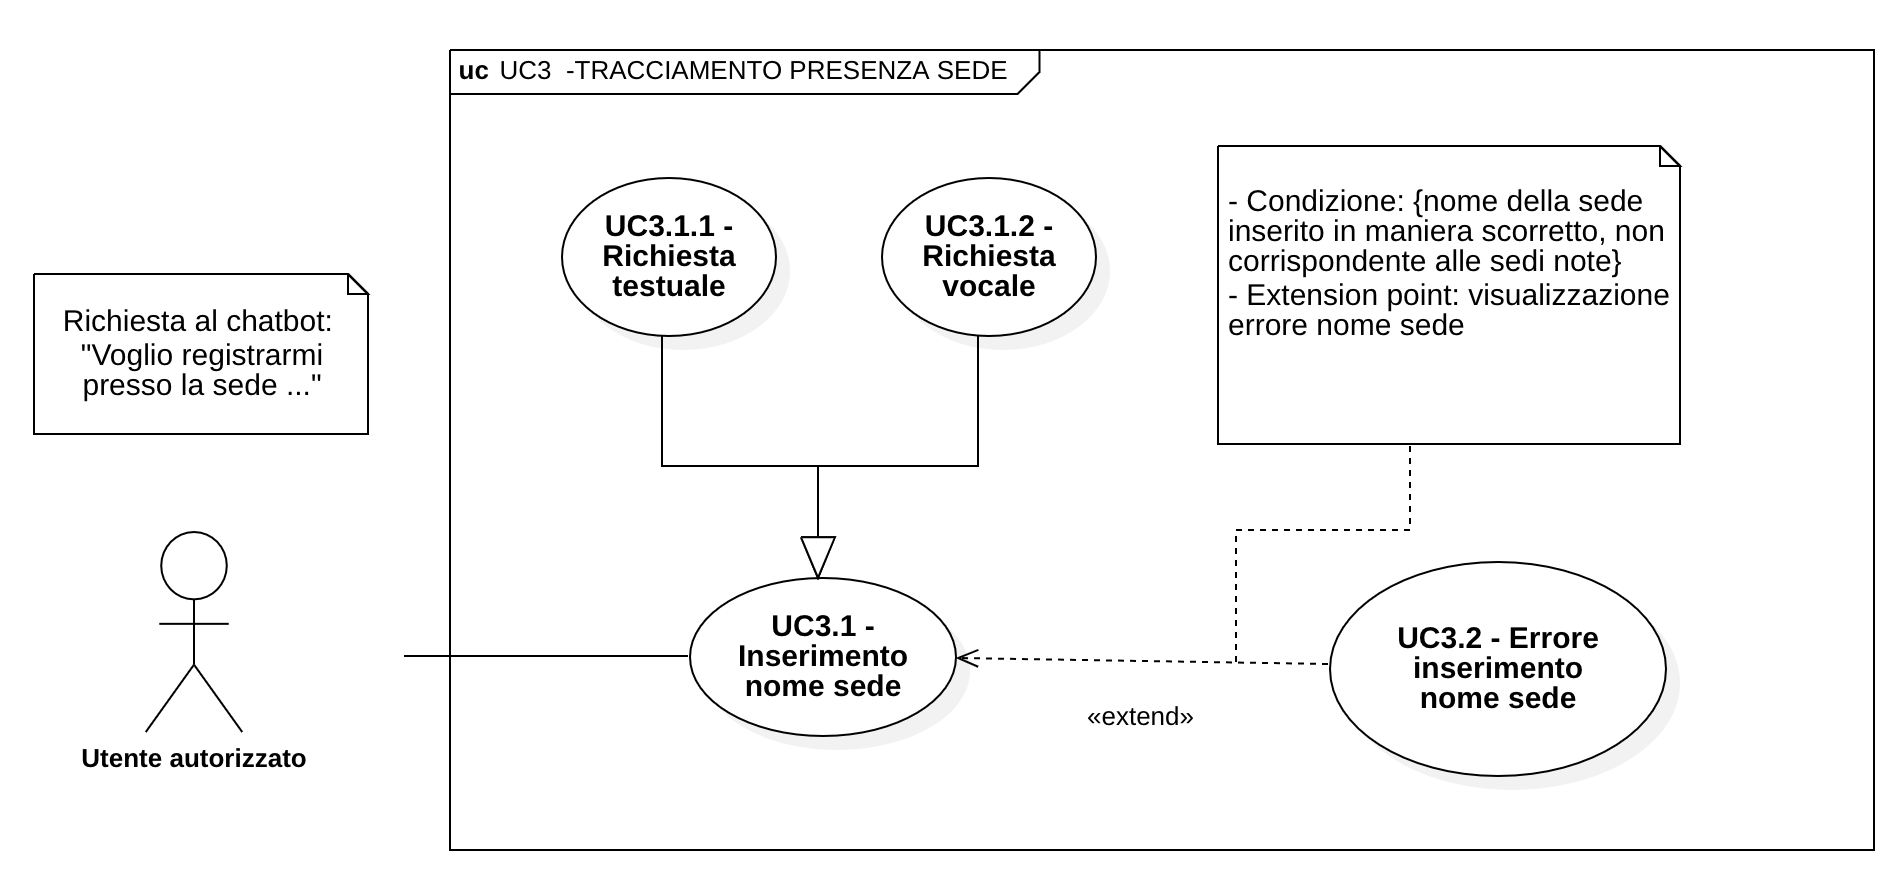
\includegraphics[scale=0.50]{images/UC2.png} 
\end{center}

\begin{itemize}
    \item \textbf{Attori}:
    \begin{itemize} 
        \item \textit{Primari}: utente autorizzato
        \item \textit{Secondari}: non presenti
    \end{itemize}
 \item \textbf{Precondizione}: l'utente (precedentemente autenticato) sta scambiando una serie di messaggi con il chatbot con lo scopo di eseguire una determinata azione.
 \item \textbf{Postcondizione}: il chatbot non è stato in grado di comprendere la richiesta dell'utente restituendo un messaggio di errore seguito da un insieme di comandi che è invece in grado di riconoscere.   
 \item \textbf{Scenario principale}: 
    \begin{itemize}
        \item Utente manda un messaggio al chatbot al fine di compire l'azione richiesta
        \item Chatbot non è in grado di interpetare ciò che gli è stato chiesto 
        \item Chatbot restituisce un messaggio di errore e suggerisce alcuni comandi che l'utente può utilizzare
    \end{itemize}
\end{itemize}